\documentclass{beamer}

\usetheme{Madrid}
\usecolortheme{beaver}

\hypersetup{
    colorlinks=true,
    linkcolor=darkred,
    filecolor=magenta,      
    urlcolor=darkred,
    pdftitle={GHC's JavaScript Backend},
    pdfpagemode=FullScreen,
    }

\AtBeginSection[]
{
  \begin{frame}
    \frametitle{Table of Contents}
    \tableofcontents[currentsection]
  \end{frame}
}

\title{GHC's JavaScript Backend}
\author{Sylvain HENRY}
\institute[IOG]{
\includegraphics[scale=0.2]{images/iohk-logo.png}}
\date[2023-06-09]{GHC Workshop\\7-9 June 2023}

\begin{document}

\frame{\titlepage}

\begin{frame}
\frametitle{Table of Contents}
\tableofcontents
\end{frame}

\section{Why?}

\begin{frame}
\frametitle{2023: Haskell in the browser}
\begin{itemize}
\item GHC 9.6: 2 new backends arrived at once
\item WebAssembly backend
\begin{itemize}
\item Cf Yesterday’s presentation by Cheng Shao
\end{itemize}
\item JavaScript backend 
\begin{itemize}
\item This presentation
\end{itemize}
\end{itemize}
\end{frame}

\begin{frame}
\frametitle{What Web backends bring to Haskell developers}
\begin{itemize}
\item Front-end Web programming
\item Standalone applications (portable, with a GUI)
\begin{itemize}
\item Node.JS engine bundled with Web rendering engine
\item e.g. ElectronJS, NW.JS…
\end{itemize}
\end{itemize}

\hspace{1cm}

\begin{itemize}
\item Two things that current Haskell ecosystem is bad at!
\begin{itemize}
\item E.g. rated “immature” on the
\href{https://github.com/Gabriella439/post-rfc/blob/main/sotu.md}{State of Haskell Ecosystem} wiki page
\end{itemize}
\item What’s really new: directly available from stock GHC
\begin{itemize}
\item Not from external projects such as GHCJS or Asterius
\end{itemize}
\end{itemize}
\end{frame}

\begin{frame}
\frametitle{Potential IOG use cases}
\begin{itemize}
\item Code reuse
\begin{itemize}
\item Cardano blockchain network nodes written in Haskell
\item Reuse code to implement clients accessing the network
\item e.g. standalone GUI wallets, Web wallets
\end{itemize}
\item Full-stack Haskell for smart contracts
\begin{itemize}
\item Smart contracts fully written in Haskell
\item One part compiled to blockchain IR
\item Other part compiled to JS/Wasm to run into users’ wallets (UI)
\end{itemize}
\end{itemize}
\end{frame}


\begin{frame}
\frametitle{ JS vs Wasm backend: do we really need both?}
\begin{center}

\includegraphics[scale=0.2]{images/js_vs_wasm.png}
\end{center}
\begin{itemize}
\item Different targets, different implementations, different trade-offs
\item JavaScript backend’s peculiarities
\begin{itemize}
\item It has its own Runtime System written in JavaScript
\item It’s the first GHC backend to target a managed platform
\item JavaScript code is human readable and can be easily tinkered with and its execution observed
\item GHCJS already proved that it can be used in production (lower risk)
\end{itemize}
\end{itemize}
\end{frame}


\begin{frame}
\frametitle{JS backend: a different RTS written in JS}

\begin{columns}

\begin{column}{0.7\textwidth}
\resizebox{8cm}{!}
{
\begin{tabular}{ll}
\hline
\textbf{Backend or project} & \textbf{Runtime System (RTS)} \\ \hline
NCG, C, and LLVM backends & C \\
JS backend, GHCJS         & JS \\
Asterius                  & JS (not the same) \\
Wasm backend & C (compiled to Wasm) \\ \hline
\end{tabular}
}
\end{column}

\begin{column}{0.2\textwidth}

\includegraphics[scale=0.3]{images/queue_rts.png}
\end{column}
\end{columns}

\vspace{1cm}

\begin{itemize}
\item Find bugs
\begin{itemize}
\item JS backend already found one bug (in some code generated by Alex)
\item Simply because out-of-bound memory accesses raise exceptions in JS
\item In the past, GHCJS similarly found bugs in the STM implementation
\end{itemize}
\item Full control
\begin{itemize}
\item The backend doesn’t rely on external tooling to convert from C to JS
\item We can write the JS code exactly as we want
\item Analogous to NCG vs C backends for codegen
\end{itemize}
\end{itemize}
\end{frame}


\begin{frame}
\frametitle{JS backend: first to target a managed platform}
\begin{itemize}
\item “Managed platform”: own heap, heap objects, and garbage collector
\item Implies changes:
\begin{itemize}
\item No pointers
\begin{itemize}
\item Addr\# isn’t represented with a number in JavaScript
\end{itemize}
\item Foreign heap objects need to be representable in Haskell codes
\begin{itemize}
\item We probably need a new ManagedRef\# primitive type
\end{itemize}
\item C FFI imports should be avoided or avoidable
\begin{itemize}
\item E.g. by providing fallback Haskell code (e.g. ghc-bignum’s native backend)
\end{itemize}
\end{itemize}
\item All of this will be useful for some future backends too!
\begin{itemize}
\item It should be easier to implement JVM and CLR (.Net) backends after this
\end{itemize}
\end{itemize}
\end{frame}


\begin{frame}
\frametitle{JS backend: observability \& tinkering}

\begin{itemize}
\item Full control of the toolchain 
\begin{itemize}
\item No LLVM, wasi-sdk, assembler, linker…
\item No limitation due to external factors
\end{itemize}
\item Reuse JS tools
\begin{itemize}
\item E.g. we already used JS profilers to find some hotspots
\end{itemize}
\item JavaScript is interpreted and readable
\begin{itemize}
\item Observe and dump anything, even interactively
\end{itemize}
\end{itemize}
\end{frame}


\begin{frame}
\frametitle{Demo: SumOfInt64}
\begin{itemize}
\item Show sources
\item Build
\item Present artefacts
\item Load in Chromium perf debugger
\item Load in Firefox perf debugger
\end{itemize}
\end{frame}

\section{Relation to GHCJS}

\begin{frame}
\frametitle{GHCJS: overview}
\begin{itemize}
\item Independent project (github.com/ghcjs)
\item Haskell to JavaScript compiler
\item Supports full Haskell (threads, Template Haskell, finalizers…)
\begin{itemize}
\item Compared to alternatives like Fay or Haste
\end{itemize}
\item Developed since $\sim$2010
\item Used in production
\item Relies on a fork of GHC 8.x
\end{itemize}
\begin{center}
\alert{The JS backend reuses code from GHCJS}
\end{center}
But why did we need the JS backend in the first place if we had GHCJS?
\end{frame}

\begin{frame}
\frametitle{GHCJS main issues and JS backend current status}
\begin{itemize}
\item[]

\includegraphics[height=1em]{images/check_green.png}
GHCJS is difficult/impossible to install (without Nix):

\item[]

\includegraphics[height=1em]{images/check_green.png}
GHCJS is stuck on old GHC

\item[]

\includegraphics[height=1em]{images/check_green.png}
GHCJS lacks CI

\item[]

\includegraphics[height=1em]{images/arrow-up-right-yellow.png}
GHCJS lacks documentation

\item[]

\includegraphics[height=1em]{images/arrow-up-right-yellow.png}
GHCJS is too slow

\item[]

\includegraphics[height=1em]{images/arrow-up-right-yellow.png}
GHCJS lacks maintainers

\item[]

\includegraphics[height=1em]{images/arrow-down-right-red.svg.png}
GHCJS produces code that is too big

\end{itemize}
\end{frame}


\begin{frame}
\frametitle{Maintainers}
\begin{columns}

\begin{column}{0.6\textwidth}
GHCJS’ maintainers
\begin{itemize}
\item Victor Nazarov (2010)
\item Hamish Mackenzie (2011-2013)
\item Luite Stegeman (2012-2021)
\end{itemize}

JS backend’s maintainers (IOG team)
\begin{itemize}
\item Jeffrey Young
\item Josh Meredith
\item Luite Stegeman
\item Sylvain Henry
\end{itemize}
\end{column}

\begin{column}{0.4\textwidth}
\begin{center}

\includegraphics[scale=0.3]{images/xkcd_2347.png}
\tiny\url{https://xkcd.com/2347/}
\end{center}
\end{column}

\end{columns}

\end{frame}


\begin{frame}[fragile]
\frametitle{Building GHC with the JS backend}
\begin{itemize}
\item Nearly identical to building native GHC
\item You need the Emscripten toolchain
\begin{itemize}
\item Used for emconfigure script, platform constants, hsc2hs…
\end{itemize}
\end{itemize}

\vspace{1cm}

\texttt
{\footnotesize
\$ ./boot \\
\$ \alert{emconfigure} ./configure -{}-target=\alert{javascript-unknown-ghcjs} \\
\$ ./hadrian/build --flavour=default+no\_profiled\_libs+\alert{native\_bignum} -j \\
\vspace{0.5cm}
\textit{wait $\sim$30 minutes, depending on your hardware} \\
\vspace{0.5cm}
\$ alias ghc-js=`pwd`/\_build/stage1/bin/javascript-unknown-ghcjs-ghc\\
}
\end{frame}


\begin{frame}
\frametitle{Code size regression}
\begin{itemize}
\item We didn’t fully port GHCJS’ JS optimizer
\begin{itemize}
\item Reason: was slow and brittle; needed redesign and rewrite
\end{itemize}
\end{itemize}
\hspace{1cm}
\begin{center}
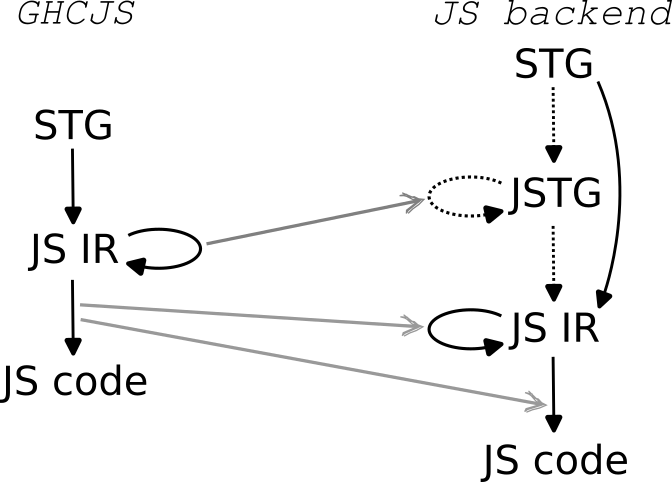
\includegraphics[scale=0.4]{images/pipelines.png}
\end{center}
\end{frame}

\section{Roadmap and status}

\begin{frame}
\frametitle{GHCJS upstreaming process(es)}

\begin{itemize}
\item Before 2022: make GHCJS converge towards GHC
\begin{itemize}
\item Avoid Template Haskell: e.g. replace JMacro QuasiQuoters
\item Only use boot libs: e.g. replace \texttt{lens}
\item Upgrade fork from GHC 8.6 to GHC 8.10
\end{itemize}

\item Since 2022: consider GHCJS as a prototype; implement a proper JS backend reusing GHCJS’ code
%\begin{itemize}
%\item Port code generator
%\item Port linker
%\item Setup CI for the JS backend (pass testsuite)
%\item Reuse GHC’s utilities: pretty-printer, binary serializer…
%\item Reimplement Template Haskell support
%\item … many other intermediate steps (500+ commits squashed into the initial commit)
%\end{itemize}
\end{itemize}
\end{frame}

\end{document}
